
\chapter{Journal}
\section{Random}

\subsection*{Who is François Chollet?}
\begin{itemize}
\item
	works on deep learning at Google in Mountain View, CA.
\item
	creator of the Keras deep-learning library
\item
	contributor to the TensorFlow machine-learning framework.
\item
	wrote a book on deep learning that is very applied rather than theoretical.
\end{itemize}

\begin{quote}
``We know the field is fast moving. If the reader looking for more recent free reading resources, there are some good introductory/tutorial/survey papers on Arxiv; I happen to be compiling a list of them''. - Auto Snipe
\end{quote}

 One of said review papers \cite{raghu2020survey}


\hrule
\section{Algo Trading}

\subsection{ML Finance Project}

\paragraph*{Terms to Learn: } NLP, bag of words, stop words, stemming, tokenizing, term-frequency inverse document frequency, bigrams, unigrams, Dow Jones Industrial Average (DJIA) index

\begin{quotation}
	`` The preprocessing for the text data involved three parts: removing stop words, stemming, and tokenizing. I first removed common words like "the" and "a". This also included removing non-standard english words, such as emojis and words in other languages. The next step was performing stemming, which turns words like "running" to "run". From there, I tried many methods of tokenizing the corpus, including bag of words, term frequency–inverse document frequency, and using bigrams and unigrams. For this particular dataset, a bag of words model using unigrams worked the best.

	Using our data from the bag of words model, I merged each day with whether or not the Dow Jones Industrial Average (DJIA) index will move up or down for the next day. I thought the movement of the DJIA would able to capture the health of the overall economy while not giving too much information into how tech stocks are specifically doing...

	The top words associated with DJIA moving up are "gadafi", "Iran" and "sanctions". ''
\end{quotation}


\subsection{\href{https://stackabuse.com/time-series-prediction-using-lstm-with-pytorch-in-python/}{Time Series in Pytorch | Introductory Example}}

\begin{quest}
	\item
	\cloze
	Neural networks can be constructed using the \pyth{torch.nn} package.

	\item
	Import the package for constructing neural networks in PyTorch.
	\begin{ans}
		\pyth{import torch.nn as nn}
	\end{ans}

	\item \cloze Seaborn comes with built-in datasets.

	\item Load seaborn's flights dataset.
	\begin{ans}
		\pyth{flight_data = sns.load_dataset("flights")}
	\end{ans}

	\item
	Why must time series data be scaled for sequence predictions?
	\begin{ans}
		When a network is fit on unscaled data, it is possible for large inputs to slow down the learning and convergence of your network and in some cases prevent the network from effectively learning your problem.
	\end{ans}

	\item
	sklearn import for scaling data?
	\begin{ans}
		\pyth{from sklearn.preprocessing import MinMaxScaler}
	\end{ans}
\end{quest}

\section{Daily Schedule (when free)}

Lex Fridman posted a video today (2020 Aug 27), detailing  \href{https://youtu.be/0m3hGZvD-0s}{his daily} schedule outside of work commitments. The stages are as follows:

\begin{tabular}{lllll}
	(1) Morning & (2) Mantra  &  (3) Deep work I & (4) Medium depth  & (5) Exercise \\
	(6) Shower & (7) Deep work II & (8) Eat & (9) Shallow work  & (10) Paper reading \\
\end{tabular}

I'll go into a bit more depth on the sections below and try to implement some of these practices in my daily schedule to see what I can learn from Lex.

\begin{enumerate}
\item
	Morning

\item
	Mantra / Daily Review
	\begin{itemize}
	\item
		Rules \& constraints
	\item
		Gratitude
	\item
		Long-term goals
	\item
		Short-term goals
	\item
		Core principles
	\end{itemize}

\item
	Deep Work I (4 hr)

\item
	Social Media and Music Practice

\item
	Exercise

	Exercise every day, no matter what. Even if injured, find a body part and exercise it.

\item
	Shower

\item
	Deep Work II (4 hr)

\item
	Eat

	2k calories, all your nutrients
	vegetables, protein, and fat

\item
	Shallow Work (1 hr)

\item
	Paper Reading (1 hr)
\end{enumerate}


\chapter{2020}

\section*{10-18-2020}
% to include all pages
%\includepdf[pages=-]
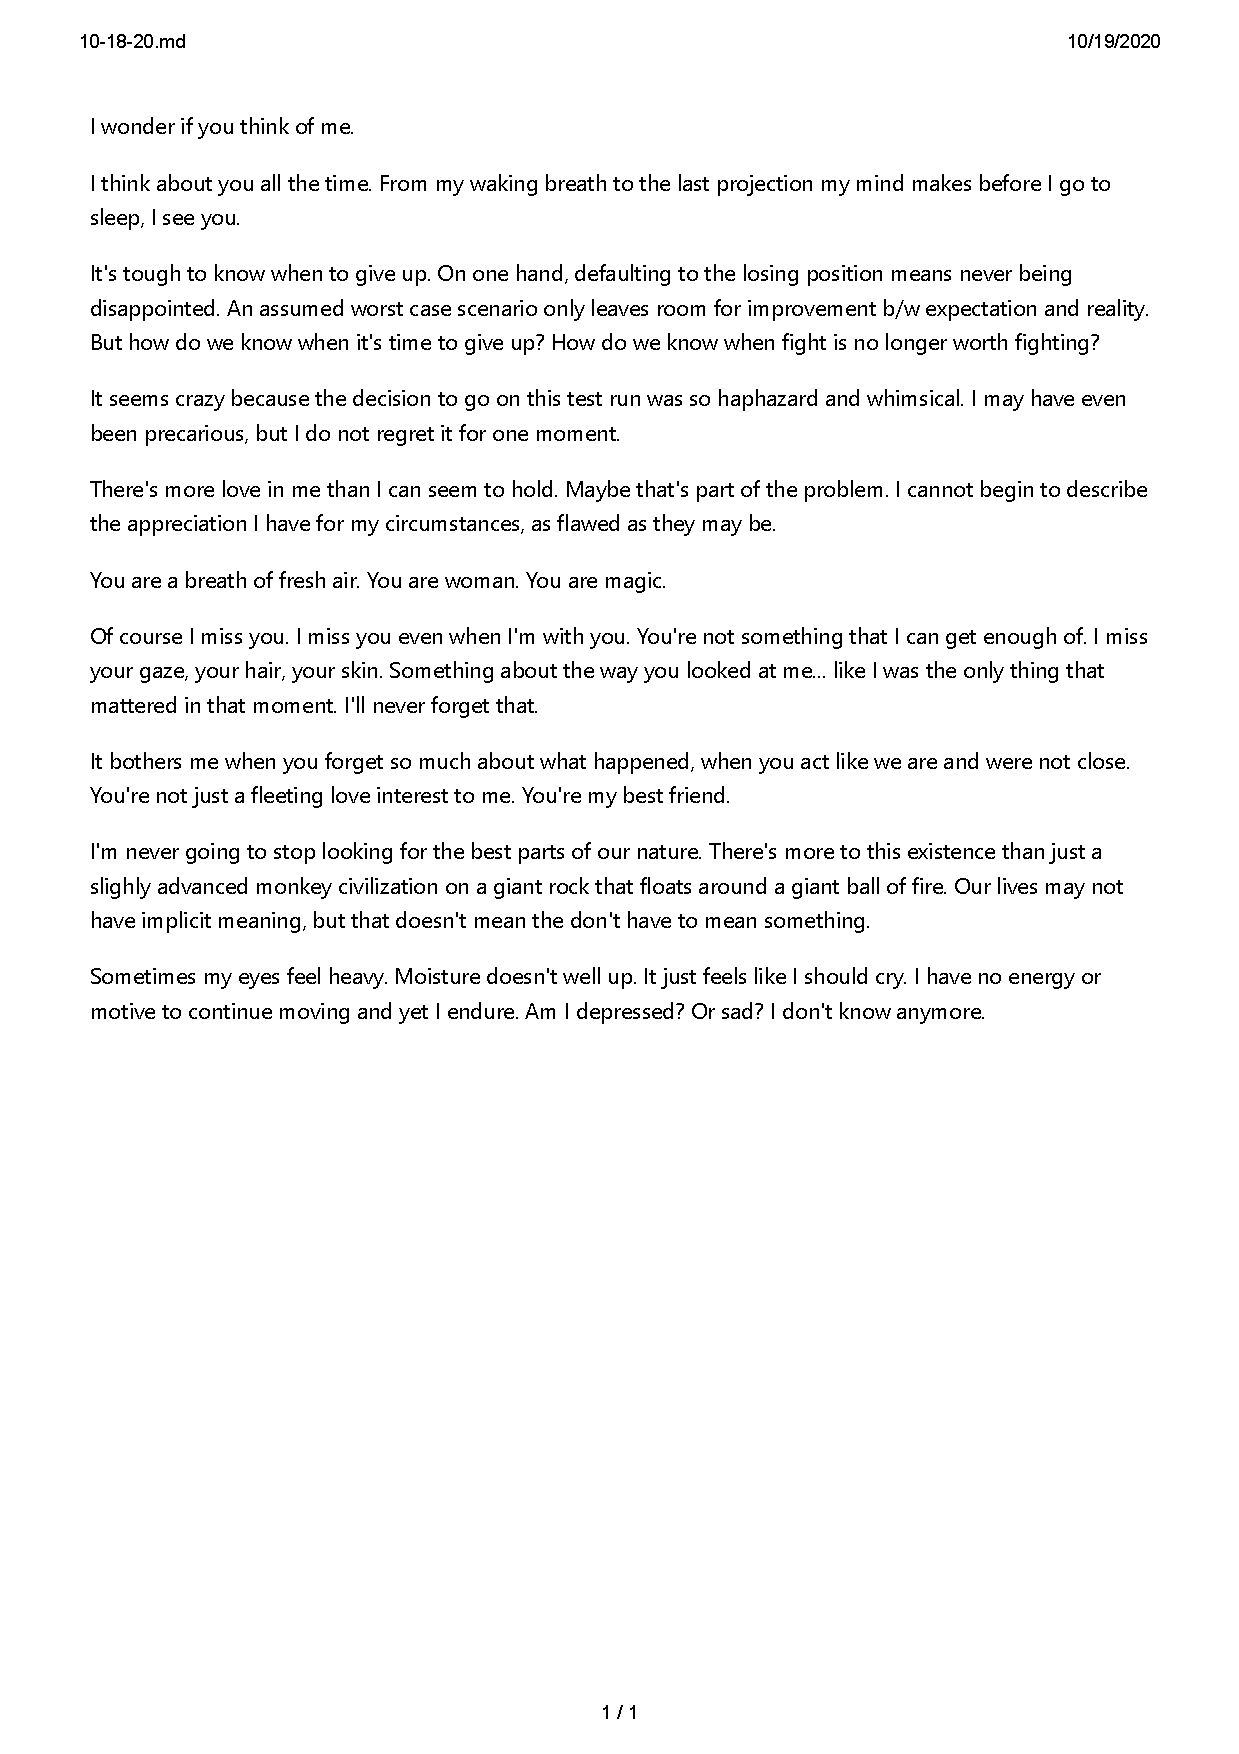
\includepdf[pages={1}]{subjects/entries/10-18-20.pdf}




